% case name
\chapter{Lock-exchange}
%
% - Purpose & Description:
%     These first two parts give reader short details about the test case,
%     the physical phenomena involved, the geometry and specify how the numerical solution will be validated
%
\section{Purpose}
%
This test demonstrates the ability of \telemac{3d} to model the motion
of two fluids with different densities.
%
\section{Description}
%
This validation case consists of a lock-exchange flow in a rectangular cavity of height
$L$ and length $7.5L$. The width of the cavity is equal to $0.3L$.
The flow consists of fresh water (on the right) and saline water (on the left)
separated at $t=0$ and suddenly released.
The heavy fluid sinks below the lighter one by forming a saline wedge which,
according to the observations, makes an angle of about $\pi/3$ with the bottom \cite{Benjamin1968}.
For this test-case, the dimensionless time is defined by:
\begin{equation}
t^+= \frac{t U}{L}
\end{equation}
with:
\begin{equation}
U = \sqrt{|\beta| S gL}
\end{equation}
Where $S$ is the salinity in the left-side of the cavity at $t=0$ and
$\beta$ the coefficient of haline dilatation.
$U$ is an estimation of the front velocity. Considering that the whole potential energy of the initial conditions is
transformed into kinetic energy, it can be estimated that the front velocity is equal to 0.5$U$.
Measurements actually show that the velocity of the lower front is about equal to $0.47U$,
while that of the upper front is about equal to $0.59U$ for a free-surface lock exchange flow \cite{Barr1967}.
The dimensionless numbers describing the flow are the Grashof number
and the Schmidt number, defined by:
\begin{equation}\label{eq:Grashof}
  Gr = \dfrac{U^2 L^2}{\nu^2}
\end{equation}
and:
\begin{equation}\label{eq:Schmidt}
  Sc =  \dfrac{\nu}{K}
\end{equation}
where $\nu$ is the molecular dynamic viscosity and $K$ is the molecular
haline diffusion coefficient. The density law depending on salinity used in TELEMAC-3D reads:
\begin{equation}
\rho = \rho_{0} (1 + 750.10^{-6} S ),
\rm{with }~ \rho_{0} = 999.972~\rm{kg/m}^3
\end{equation}
so that $\beta$ is equal to $-7.5.10^{-4}~(\text{g/L})^{-1}$.

% Preample
\section{Preamble -- an attempt at reproducing Adduce \textit{et al.}'s experiments}\label{sec:adduce}

In order to compare the shape of the simulated flow to experimental results,
we first considered the case studied experimentally by Adduce \textit{et al.} \cite{Adduce2012}.
A $t^+=0$, the separation between the fresh and saline water is now located at
$L$ from the left side of the cavity.
The Schmidt number is still equal to 1 but the Grashof number is now
equal to $7.3.10^{8}$ (the salinity is set to 9~g/L in the left part and 0~g/L on the right part,
the molecular dynamic viscosity is set to $2.7.10^{-5}m^2s^{-1}$).
The non-hydrostatic version of TELEMAC-3D was used, using an N
advection scheme with the option 2 and 5 corrections.
The dynamic pressure is calculated before the resolution of the
wave equation and no turbulence model is used.
The figure \ref{fig:lock_adduce_dp_yes_PSI2_5corr} shows the
results obtained at $t^+=$ 7.3 and 16.4 compared to the experiments.
The velocity of the front seems correctly reproduced by the numerical model,
but the shape of the flow is quite different from the experimental one.
The simulation was run without using any turbulence model,
which may explain why there is less diffusion than in the experiment.
\begin{figure}[ht]
  \begin{center}
    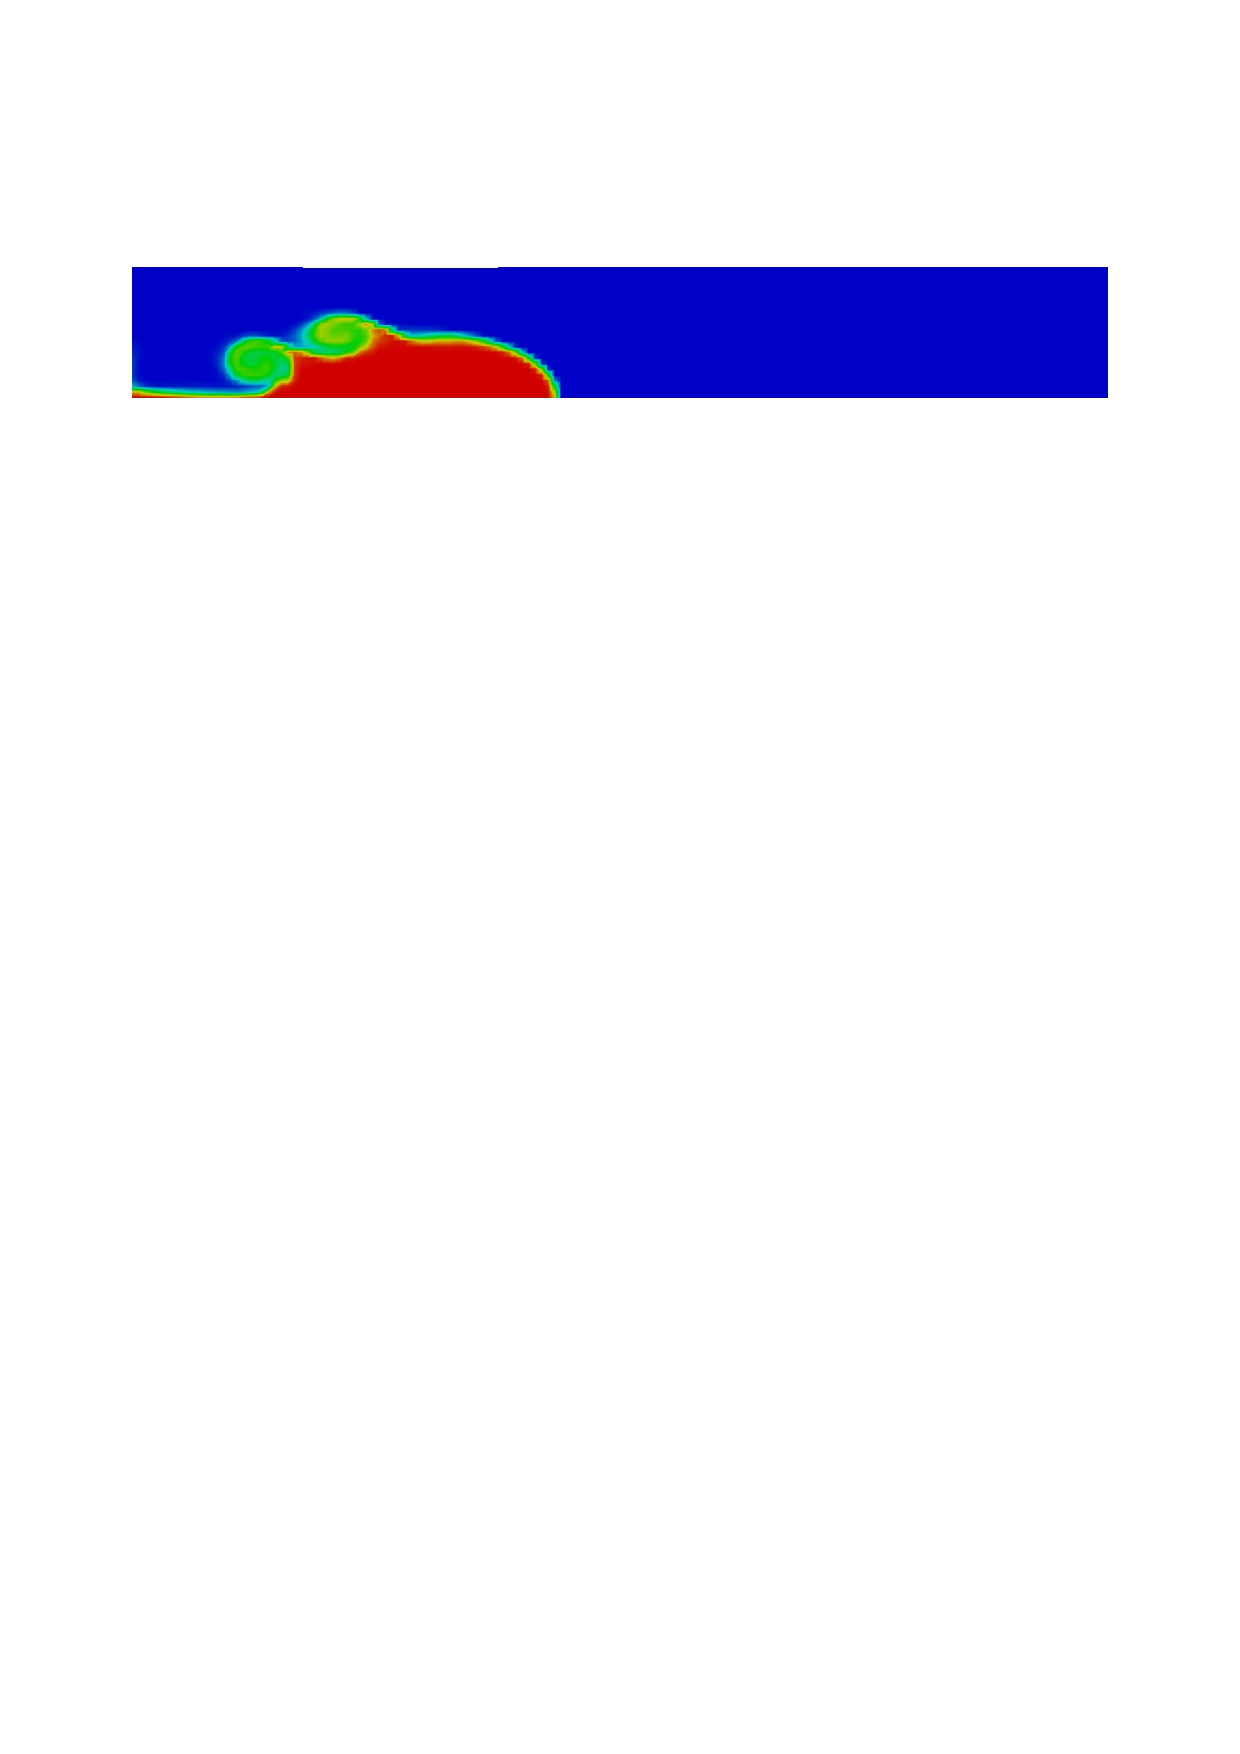
\includegraphics[scale=0.41, trim=40 648 0 50, clip]{./img/lock_adduce_4_dp_yes_PSI2_5corr.pdf} \hspace{-0.7cm}
    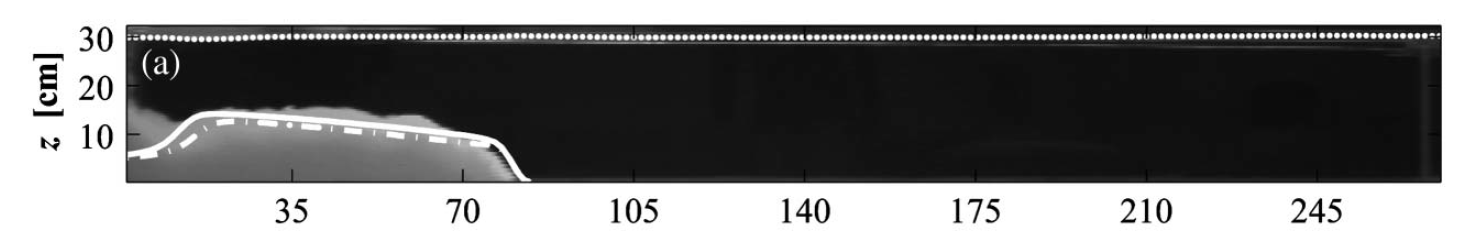
\includegraphics[scale=0.22, trim=88 30 180 0, clip]{./img/adduce_4.png} \vspace{-0.1cm}\\
    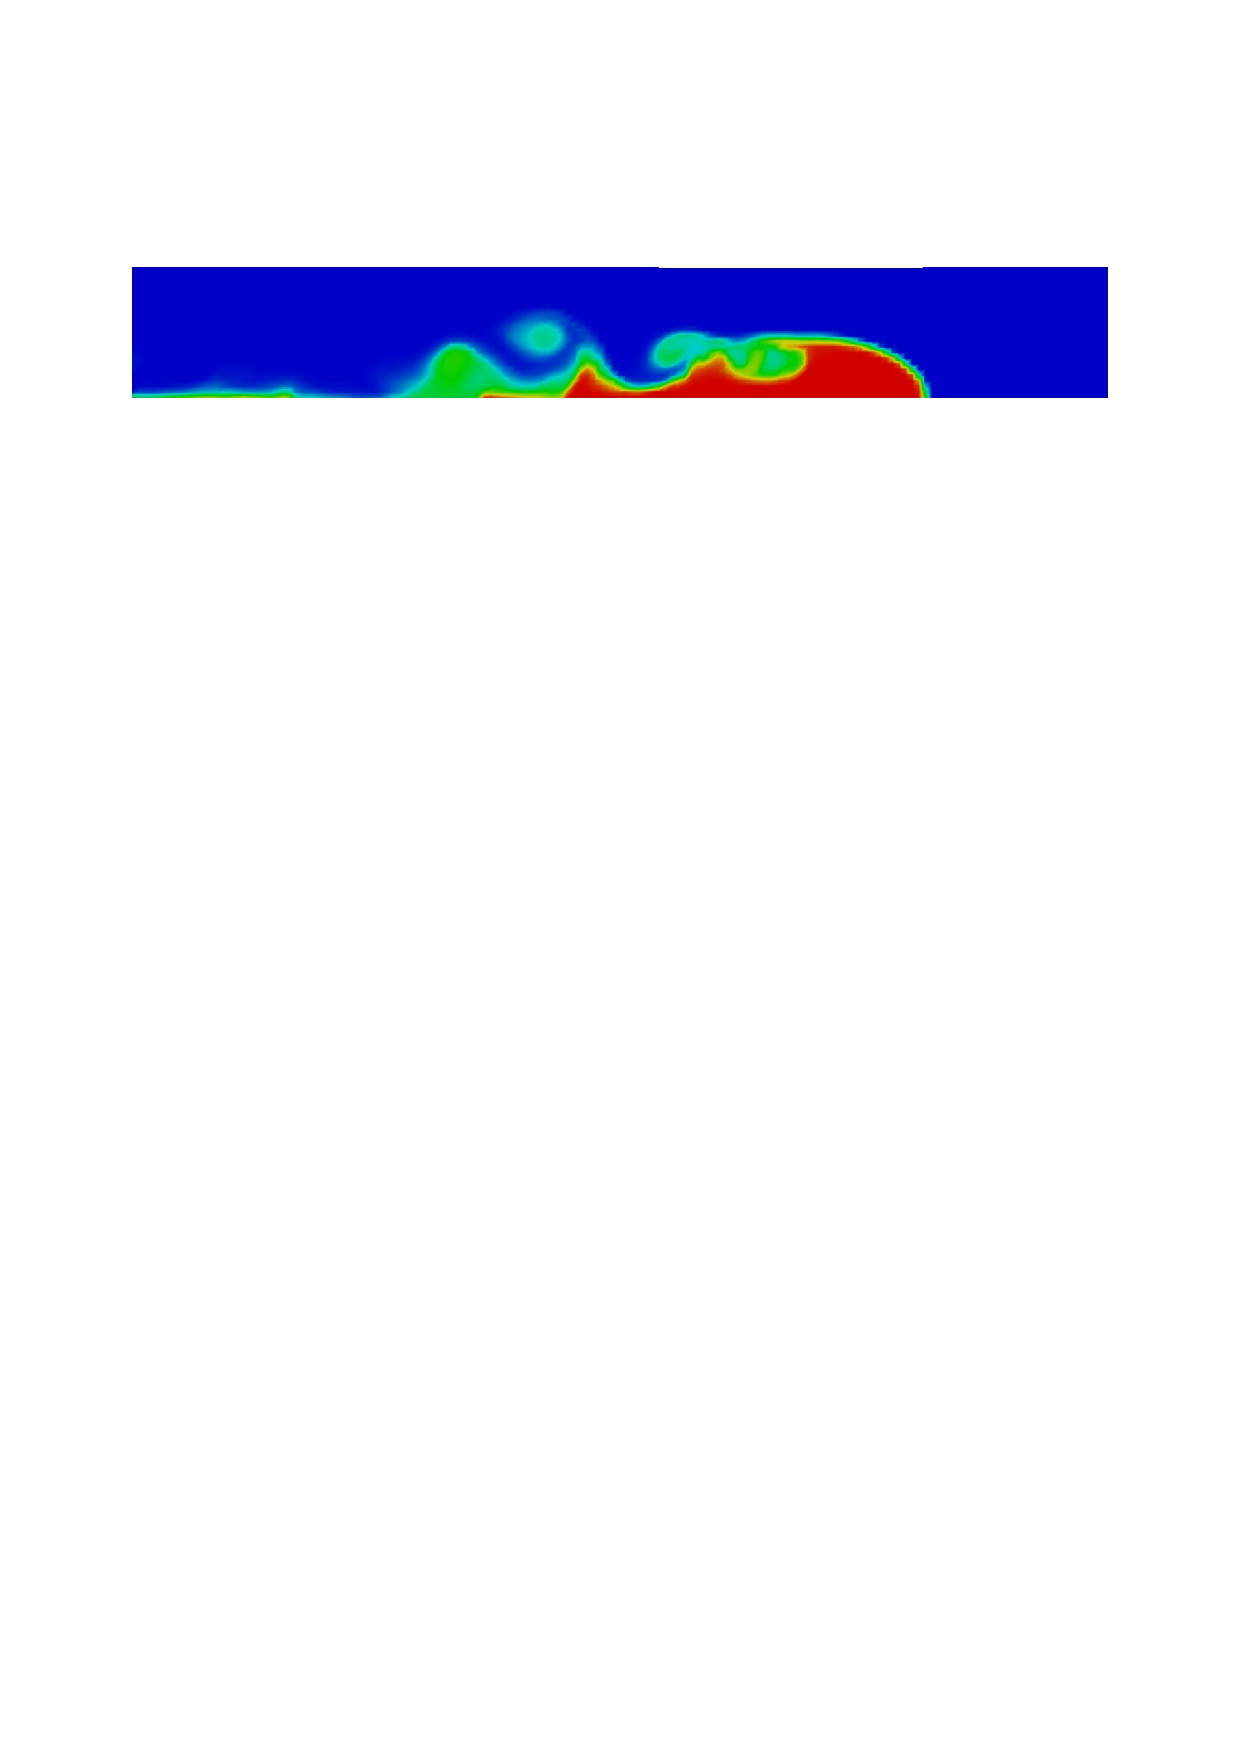
\includegraphics[scale=0.41, trim=50 648 0 100, clip]{./img/lock_adduce_9_dp_yes_PSI2_5corr.pdf} \hspace{-0.7cm}
    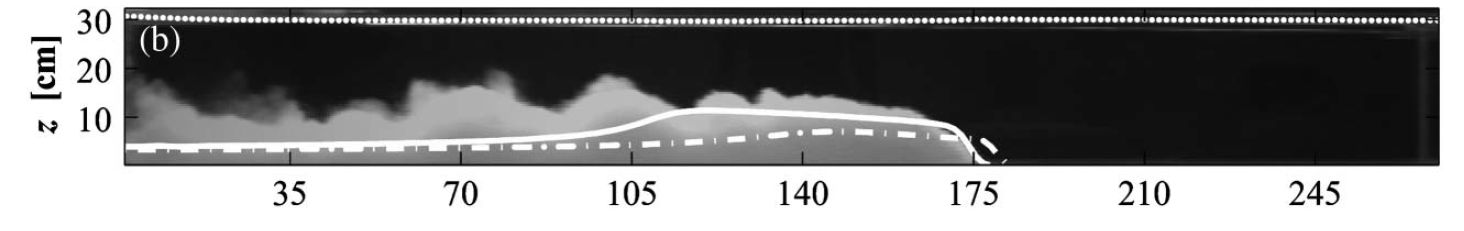
\includegraphics[scale=0.22, trim=88 40 165 0, clip]{./img/adduce_9.png}
    \caption{Lock-exchange: comparison of the experimental results by Adduce \textit{et al.} \cite{Adduce2012} (right)
      at $t^+=7.3$ and $16.4$ with the simulation results (left),
      using a N advection scheme with the option 2 and 5 corrections.
      The dynamic pressure is calculated before the resolution of the wave equation.}
    \label{fig:lock_adduce_dp_yes_PSI2_5corr}
  \end{center}
\end{figure}

The same simulation was then run with the $k-\epsilon$ turbulence model applied in all directions,
but there is no visible impact on the results because this is a case of transition
between a laminar and a turbulent flow.
In these conditions, it is hard to compare the various advection
schemes or numerical options on this case:
different flow shapes are obtained but there is never enough
diffusion to match the turbulent diffusion observed in the experiments.
We did not find reference data regarding a less turbulent
experimental setup where the shape of the free-surface flow is displayed.
Thus, we chose to simulate a case without available
experimental data but with a lower Grashof number.

\section{Case setup}

\subsection{Geometry and mesh}
%
Given the difficulties in reproducing a free-surface experimental setup, the case simulated here is
the one described in J. Jankowski's PhD thesis \cite{Jankowski1999}.
The flow consists of fresh water (on the right) and saline water (on the left)
separated at $t^+=0$ at the half-width of the domain.
The Schmidt number is equal to 1 and the Grashof number is equal to $8.10^{7}$
(the salinity is set to 1~g/L in the left part and 0~g/L on the right part,
the molecular dynamic viscosity is set to $2.7.10^{-5}m^2s^{-1}$).
%
\subsubsection{Bathymetry}
%
The bed of the cavity is flat at the elevation $z$ = -4~m.
%
\subsubsection{Geometry}
%
The cavity is 30~m long and 1.2~m wide.
%
\subsubsection{Mesh}
%
The mesh consists of 1,806 triangular elements, which corresponds to 1,060 nodes.
Along the vertical, 24 regularly spaced planes are used.
The figure \ref{fig:lock-mesh} shows a vertical and a horizontal section of the mesh.
\begin{figure}[ht]
  \begin{center}
        \includegraphicsmaybe{[scale=0.3, trim=35 20 0 0, clip]}{../img/lock_mesh_vertical.png}
        \includegraphicsmaybe{[scale=0.3, trim=35 20 0 0, clip]}{../img/lock_mesh_horizontal.png}
        \caption{Lock-exchange: vertical (top) and a horizontal (bottom) sections of the mesh.}
    \label{fig:lock-mesh}
  \end{center}
\end{figure}
%
%
% - Physical parameters:
%     This part specifies the physical parameters
%
%
\subsection{Physical parameters}
%
The influence of the Coriolis force and meteorological forcings
are not taken into account.
%
% Reference results

\subsection{Initial and Boundary Conditions}
%
\subsubsection{Initial conditions}
%
- Constant water depth = 4~m\\
- No velocity\\
- Initial salinity: 1~g/L on the left half part and 0~g/L in the other
part (defined in the subroutine \telfile{T3D\_CONDIM} and the keyword
\telkey{INITIAL VALUES OF TRACERS}) -- see the figure \ref{fig:lock-initial_salinity}.
\begin{figure}[ht]
  \begin{center}
        \includegraphicsmaybe{[scale=0.3, trim=35 20 0 0, clip]}{../img/lock_initial_salinity.png}
        \caption{Lock-exchange: initial salinity distribution, ranging from 0 (blue)
          to 1 (red).}
    \label{fig:lock-initial_salinity}
  \end{center}
\end{figure}
%
\subsubsection{Boundary conditions}
%
- Closed boundaries\\
- No bottom friction
%
\subsection{General parameters}
%
- Time step: 0.5~s\\
- Simulation duration: 100~s
%
% - Numerical parameters:
%     This part is used to specify the numerical parameters used
%     (adaptive time step, mass-lumping when necessary...)
%
%
\subsection{Numerical parameters}
%
- Advection of velocities and tracers: tests with the characteristics scheme, SUPG,
the Leo-Postma scheme and the N and PSI-type MURD schemes with options 1, 2 and 3 and several numbers of corrections\\
- DYNAMIC PRESSURE IN WAVE EQUATION: runs with this key-word set to YES and NO
(dynamic pressure calculated before and after the wave equation resolution, respectively)\\
- Linear solver: solver 7 (GMRES) used with a precision of $10^{-10}$ and a maximum of 2000 iterations for all the matrix inversions\\
- Implicitation coefficients on the velocity and depth : 0.5\\
- Non-hydrostatic version: used to test the advection schemes and dynamic pressure option, one hydrostatic run also performed to
compare to the non-hydrostatic version
%
%
% - Reference results
%
%
\section{Reference results}

There is no available experimental data regarding the shape of the flow for
this specific case, but we have an estimation of the angle between the wedge and the bottom and the
front velocity values. The angle should be about equal to $\pi/3$ and the lower front
velocity should be about equal to $0.081$m/s.
On this case, it is also expected that Rayleigh-Taylor instability cells will form at the interface between the two fluids.
In order to have an idea what these instabilities should look like, fine simulations were run
with the second order predictor-corrector PSI MURD-type advection scheme
(the most accurate advection solver in TELEMAC-3D at the moment -- SCHEME OPTION FOR THE ADVECTION 3).
The triangle size in the horizontal mesh is 0.025m and 80 planes are used,
so that the horizontal and vertical discretisations are equal.
The 3D mesh contains about 9 million points. The time step size is equal to 0.2~s
and the simulation duration is 100~s ($t^+=4.29$).
The figures \ref{fig:fine_sim} and \ref{fig:fine_sim_dpwaveq} show the
results at $t^+=4.29$ when using 5, 10 and 15 corrections,
calculating the dynamic pressure after or before the resolution of the wave equation.
We observed that this option has a visible influence on the results.

\begin{figure}[ht]
  \begin{center}
    \includegraphicsmaybe{[scale=0.25, trim=35 300 0 300, clip]}{./img/lock-exchange_0,025_80p_PSI3_5corr.png}
    \includegraphicsmaybe{[scale=0.25, trim=35 300 0 300, clip]}{./img/lock-exchange_0,025_80p_PSI3_10corr.png}
    \includegraphicsmaybe{[scale=0.25, trim=35 300 0 300, clip]}{./img/lock-exchange_0,025_80p_PSI3_15corr.png}
    \caption{Lock-exchange: fine simulation results at $t^+=4.29$ with a PSI advection scheme
      with the option 3, using 5, 10 and 15 corrections (from top to bottom).
      The dynamic pressure is calculated after the resolution of the wave equation.}
    \label{fig:fine_sim}
  \end{center}
\end{figure}
\begin{figure}[ht]
  \begin{center}
    \includegraphicsmaybe{[scale=0.25, trim=35 300 0 300, clip]}{./img/lock-exchange_0,025_80p_dpwaveq_PSI3_5corr.png}
    \includegraphicsmaybe{[scale=0.25, trim=35 300 0 300, clip]}{./img/lock-exchange_0,025_80p_dpwaveq_PSI3_10corr.png}
    \includegraphicsmaybe{[scale=0.25, trim=35 300 0 300, clip]}{./img/lock-exchange_0,025_80p_dpwaveq_PSI3_15corr.png}
    \caption{Lock-exchange: fine simulation results at $t^+=4.29$ with a PSI advection scheme
      with the option 3, using 5, 10 and 15 corrections (from top to bottom).
      The dynamic pressure is calculated before the resolution of the wave equation.}
    \label{fig:fine_sim_dpwaveq}
  \end{center}
\end{figure}

The mean velocity of the lower front is equal to $0.084$~m/s and the angle between the wedge front and the
vertical is about equal to $\pi/3$, which matches experimental observations on this type of flows.
It is also visible that several instability cells appear in the simulations. At least three cells appear at the interface,
and one or two more depending on the numerical options.
The shape of the instability cells is influenced by the option DYNAMIC PRESSURE IN WAVE EQUATION
and by the number of corrections in the distributive scheme.
These results show that this case is very sensitive to slight numerical changes.
In what follows, we will compare the various advection schemes, the DYNAMIC PRESSURE IN WAVE EQUATION option and
the hydrostatic version of TELEMAC-3D on this case: for a given discretisation, we will observe whether the
main instability cells appear or not, and check the value of the angle to the bottom and of the front velocity.
%
% - Results
%
%
\section{Results}
%
\subsection{Dynamic pressure not included in the wave equation}

\subsubsection{Characteristics}

The figure \ref{fig:lock-exchange_dp_no_carac} shows the results obtained with the characteristics advection scheme at $t^+=$ 4.29.
The lower front velocity is equal to $0.072$m/s in the simulation (as compared to $0.081$m/s) and the angle of the wedge is well captured
by the model but it is so diffusive that the Rayleigh-Taylor instabilities do not trigger.
\begin{figure}[ht]
  \begin{center}
    \includegraphicsmaybe{[scale=0.3, trim=35 20 0 0, clip]}{../img/lock-exchange_CARAC.png}
    \caption{Lock-exchange: simulation result at $t^+=4.29$ with the characteristics advection scheme.
      The dynamic pressure is calculated after the resolution of the wave equation.}
    \label{fig:lock-exchange_dp_no_carac}
  \end{center}
\end{figure}

\subsubsection{SUPG}
The figure \ref{fig:lock-exchange_dp_no_SUPG} shows the results obtained with the SUPG advection scheme, with the option 2 on the velocity and tracer and the option 0 on the water depth, at $t^+=$ 4.29.
It is visible that the maximum principle is not fulfilled with this scheme since the final tracer values are outside the initial bounds.
The spurious behaviour mostly occurs at the upper and lower fronts, in the white zones of the plot.
On the other hand, the lower front velocity is equal to $0.082$m/s in the simulation (as compared to $0.081$m/s) and the angle of the wedge
is well captured by the model. It is however too diffusive to let instabilities develop during the simulation.
They are slightly visible in the results, but still very diffused.
\begin{figure}[ht]
  \begin{center}
    \includegraphicsmaybe{[scale=0.315, trim=45 20 40 0, clip]}{../img/lock-exchange_SUPG.png}
    \caption{Lock-exchange: simulation result at $t^+=4.29$ with the SUPG advection scheme with the salinity ranging from -0.1 (dark blue)
      to 1.1 (dark red) on the top and from -1.4 (blue) to 2 (red) on the bottom.
      The dynamic pressure is calculated after the resolution of the wave equation.}
    \label{fig:lock-exchange_dp_no_SUPG}
  \end{center}
\end{figure}

\subsubsection{Leo Postma scheme}
The figure \ref{fig:lock-exchange_dp_no_LP} shows the results obtained with the Leo Postma advection scheme at $t^+=$ 4.29.
The lower front velocity is equal to $0.074$m/s in the simulation (as compared to $0.081$m/s) and the angle of the wedge
is well captured by the model. The model but it is too diffusive, so that the Rayleigh-Taylor instabilities do not trigger in the simulation.
\begin{figure}[ht]
  \begin{center}
    \includegraphicsmaybe{[scale=0.3, trim=35 20 0 0, clip]}{../img/lock-exchange_LEOP.png}
    \caption{Lock-exchange: simulation result at $t^+=4.29$ with the Leo Postma advection scheme.
      The dynamic pressure is calculated after the resolution of the wave equation.}
    \label{fig:lock-exchange_dp_no_LP}
  \end{center}
\end{figure}

\subsubsection{PSI (or N) scheme}
The figures \ref{fig:lock-exchange_dp_no_PSI1} to \ref{fig:lock-exchange_dp_no_PSI3} show the results
obtained with the options 1, 2 and 3 with the PSI scheme, using two to five corrections, at $t^+=$ 4.29.
We recall that the option 1 corresponds to the classical scheme, the option 2 is the first order predictor-corrector
scheme and the option 3 is the second-order predictor corrector scheme.
The results obtained with the N scheme are very similar so they are not shown here.
It appears in the results that for this discretisation the first order predictor-corrector scheme
provides better results than the second-order one since they present more instability cells.
Both have converged after about 4 corrections.
The lower front velocity is equal to $??$m/s in the simulations (as compared to $0.081$m/s).
\begin{figure}[ht]
  \begin{center}
    \includegraphicsmaybe{[scale=0.3, trim=35 20 0 0, clip]}{../img/lock-exchange_PSI1.png}
    \caption{Lock-exchange: simulation result at $t^+=4.29$ with a PSI advection scheme with the option 1.
      The dynamic pressure is calculated after the resolution of the wave equation.}
    \label{fig:lock-exchange_dp_no_PSI1}
  \end{center}
\end{figure}
\begin{figure}[ht]
  \begin{center}
    \includegraphicsmaybe{[scale=0.3, trim=35 20 0 0, clip]}{../img/lock-exchange_PSI2_2corr.png}
    \includegraphicsmaybe{[scale=0.3, trim=35 20 0 0, clip]}{../img/lock-exchange_PSI2_3corr.png}
    \includegraphicsmaybe{[scale=0.3, trim=35 20 0 0, clip]}{../img/lock-exchange_PSI2_4corr.png}
    \includegraphicsmaybe{[scale=0.3, trim=35 20 0 0, clip]}{../img/lock-exchange_PSI2_5corr.png}
    \caption{Lock-exchange: simulation result at $t^+=4.29$ with a PSI advection scheme with the option 2,
      using 2, 3, 4 and 5 corrections (from top to bottom).
      The dynamic pressure is calculated after the resolution of the wave equation.}
    \label{fig:lock-exchange_dp_no_PSI2}
  \end{center}
\end{figure}
\begin{figure}[ht]
  \begin{center}
    \includegraphicsmaybe{[scale=0.3, trim=35 20 0 0, clip]}{../img/lock-exchange_PSI3_2corr.png}
    \includegraphicsmaybe{[scale=0.3, trim=35 20 0 0, clip]}{../img/lock-exchange_PSI3_3corr.png}
    \includegraphicsmaybe{[scale=0.3, trim=35 20 0 0, clip]}{../img/lock-exchange_PSI3_4corr.png}
    \includegraphicsmaybe{[scale=0.3, trim=35 20 0 0, clip]}{../img/lock-exchange_PSI3_5corr.png}
    \caption{Lock-exchange: simulation result at $t^+=4.29$ with a PSI advection scheme with the option 3,
      using 2, 3, 4 and 5 corrections (from top to bottom).
      The dynamic pressure is calculated after the resolution of the wave equation.}
    \label{fig:lock-exchange_dp_no_PSI3}
  \end{center}
\end{figure}

\clearpage

\subsection{Dynamic pressure included in the wave equation}

In this section we show the results obtained when the dynamic pressure is calculated
before the resolution of the wave equation (thus, before the hydrostatic pressure).
This change does not impact the results obtained with the characteristics, SUPG and Leo Postma schemes
because they are so diffusive that for this discretisation the instability cells do not appear.
However, the results obtained with the predictor-corrector PSI scheme are influenced by this option. The same holds
for the N scheme, but once again the results obtained with the N and PSI schemes were so close that
we chose to show only the results of the PSI scheme, which were even slightly improved compared to the results of the N scheme.
Here we only show the results obtained with the first-order predictor-corrector PSI scheme since
we saw previously that it provides the best results for this mesh discretisation.

\subsubsection{PSI scheme}
The figure \ref{fig:lock-exchange_dp_yes_PSI2} shows the results
obtained with the option 2 for the PSI scheme, using two to five corrections, at $t^+=$ 4.29.
\begin{figure}[ht]
  \begin{center}
    \includegraphicsmaybe{[scale=0.3, trim=35 20 0 0, clip]}{../img/lock-exchange_dpwaveq_PSI2_2corr.png}
    \includegraphicsmaybe{[scale=0.3, trim=35 20 0 0, clip]}{../img/lock-exchange_dpwaveq_PSI2_3corr.png}
    \includegraphicsmaybe{[scale=0.3, trim=35 20 0 0, clip]}{../img/lock-exchange_dpwaveq_PSI2_4corr.png}
    \includegraphicsmaybe{[scale=0.3, trim=35 20 0 0, clip]}{../img/lock-exchange_dpwaveq_PSI2_5corr.png}
    \caption{Lock-exchange: simulation result at $t^+=4.29$ with a PSI advection scheme with the
      option 2, using 2, 3, 4 and 5 corrections (from top to bottom).
      The dynamic pressure is calculated before the resolution of the wave equation.}
    \label{fig:lock-exchange_dp_yes_PSI2}
  \end{center}
\end{figure}

\clearpage

\subsection{Hydrostatic hypothesis}

The results of the hydrostatic computation are presented in the figure
\ref{t3d:lock-exchange:hydro_res}.
The average velocity of the lower front is approximately 0.068~m/s and
the angle of the wedge compared to the bottom is close to 90$^\circ$.
Besides, the instability cells do not appear in the results.
This shows that the hydrostatic hypothesis is not valid for this type of
case.
\begin{figure}[h]
  \centering
  \includegraphicsmaybe{[scale=0.3, trim=35 20 0 0, clip]}{../img/lock-exchange_hydro.png}
  \caption{Lock exchange test: results with the hydrostatic hypothesis}
  \label{t3d:lock-exchange:hydro_res}
\end{figure}
%
\section{Conclusion}
%
%\telemac{3d} simulates correctly the motion of fluids with different densities.
In this document, a sensitivity analysis on the lock-exchange case was performed.
First, we tried to reproduce an experimental setup, but realized we could not
correctly reproduce the flow shape with TELEMAC-3D: without a turbulence closure,
there is not enough diffusion in the numerical result whereas using the $k-\epsilon$
turbulence model is way too diffusive. Thus, we chose a less turbulent setup, which
is actually the one proposed in J. Jankowski's PhD thesis and was already used as a TELEMAC-3D example.
We used twice as many planes as in the original simulation, using the non-hydrostatic
version of TELEMAC-3D and testing the various advection schemes and the option DYNAMIC PRESSURE IN
WAVE EQUATION. We also compared the hydrostatic and non-hydrostatic versions.
In order to have a reference solution, fine simulations for this case were run,
with a space discretisation of 0.025m (9 million points in 3D).
The results of the fine simulations showed that Rayleigh-Taylor instabilities appear at the
interface between the two fluids. There are three major central cells and, depending on
the options, one or two smaller external cells. Their shape is influenced by the number of corrections
used in the distributive scheme and the choice for the option DYNAMIC PRESSURE IN WAVE EQUATION.\\

In the coarser simulations, we observed that only the N or PSI MURD-type
advection schemes with the option 2 (1st order predictor-corrector) or 3 (2nd order predictor-corrector)
are accurate enough to reproduce the instability cells with this discretisation (0,2m).
The 2nd order predictor-corrector PSI or N schemes have a higher order of
convergence than the 1st order one, but for this discretisation the latter
provide better results. The three main instability cells only appear when setting the option
DYNAMIC PRESSURE IN WAVE EQUATION to YES and with the 1st order predictor-corrector N or PSI schemes.
The results thus seem to be improved by calculating the dynamic pressure before the
resolution of the wave equation. We can also conclude that the options 2 or 3 for the MURD-type
advection schemes greatly improve the quality of the numerical solution provided by TELEMAC-3D
compared to all the other advection schemes.
However, it seems difficult for the user to choose the number of corrections to apply
in the distributive schemes and a possible improvement
would be to let TELEMAC-3D decide when the algorithm has converged based
on a convergence criterion. \\

On the other hand, the results show that the hydrostatic hypothesis is not valid for this type of case:
the shape of the flow is not correctly reproduced with the hydrostatic option.\\

Finally, it is important to keep in mind that this test-case is
very sensitive due to its unstable nature, and that slight changes to the schemes
might lead to significant differences when it comes to the shape of the instabilities.

